% =====================================================================
% Arquiteturas de hardware (Resultados), por condição de teste.
% Esqueleto (2026-11-07). Dados: relatórios do servidor (Vivado 2023.2),
%   hardware/resultados_servidor/.
% Tabelas e números (2026-11-08): software/testes/analise_potencia_qualidade.py
%   (tabelas em hardware/resultados_servidor/tabelas/*.tex, números em .../tabelas/resumo.txt)
%   e figuras_potencia_servidor.py (potencia_media_condicao). As tabelas foram coladas aqui;
%   ao gerar de novo, comparar com o .tex do script.
% Figuras (2026-11-09; separadas em 2026-11-13): energia_inversao (energia_inversao_formatos) e
%   potencia_recursos (potencia_recursos_lado), ambas de figuras_potencia_servidor.py, e quadrantes_cond_g1/_g3 (analise_potencia_qualidade.py), copiadas em
%   Images/RESULTADOS. Tabela tab:escolha-condicao: tabelas/tabela_escolha_condicao.tex.
% 2026-11-09: conferido depois da rodada6 (grade inteira): tabelas e figuras iguais.
% =====================================================================
% Sem isto, as figuras da seção de formatos (grupo 3 e perfis) saíam no meio desta seção.
% 2026-11-11: \FloatBarrier no lugar do \clearpage, que deixava a figura dos perfis sozinha
%   numa página.
\FloatBarrier
\section{\texorpdfstring{\textcolor{red}{Arquiteturas de hardware}}{Arquiteturas de hardware}}\label{sec:resultados-hardware}

% 2026-11-13: seção reorganizada a pedido da autora. Introdução nova; recursos primeiro por
%   arquitetura, na ordem da Metodologia (subsec:hw-arquiteturas), com o recurso mais usado e o
%   motivo; depois as tabelas e a comparação geral. Backup: scratchpad da sessão 8a590fec.
% FONTE da introdução: Tabela tab:recursos-faixa (intervalo x limite; caminho crítico).

\textcolor{red}{Esta seção mostra os resultados de implementação das arquiteturas no XCU50, a 100~MHz. Em todos os formatos, nas arquiteturas otimizadas, o intervalo entre duas inversões fica abaixo do limite de ciclos da Tabela~\ref{tab:limite-ciclos}. O módulo aceita um bloco novo de 275 matrizes a cada $T_c$ e acompanha a chegada das amostras. O timing é alcançado em todas as arquiteturas, com maior caminho crítico de 9,74~ns, na TDLB100-400.}

\textcolor{red}{A Seção~\ref{subsec:resultados-recursos-arquitetura} analisa os recursos de cada arquitetura, na mesma ordem da Seção~\ref{subsec:hw-arquiteturas}, e mostra qual recurso cada uma mais usa e por quê. A Seção~\ref{subsec:resultados-recursos} compara as arquiteturas e os formatos, e a Seção~\ref{subsec:resultados-potencia} mostra a potência e a energia por inversão.}

% ---------------------------------------------------------------------
\subsection{\texorpdfstring{\textcolor{red}{Recursos por arquitetura}}{Recursos por arquitetura}}\label{subsec:resultados-recursos-arquitetura}
% ---------------------------------------------------------------------
\textcolor{red}{A Figura~\ref{fig:recursos-faixa-arquitetura} mostra o uso de cada recurso em cada arquitetura, em porcentagem do XCU50. Cada traço vai do menor ao maior uso entre os formatos. O recurso mais usado de cada arquitetura é o traço mais alto do grupo. Nas seções a seguir, cada arquitetura é comparada com a anterior. Quando o texto diz, por exemplo, que as LUTs crescem de 4,6 a 6,8 vezes, a conta é feita com o mesmo formato nas duas arquiteturas, e a faixa vai do formato que cresce menos ao que cresce mais (Tabelas~\ref{tab:recursos} e \ref{tab:recursos-sem-otimizacao}).}

\begin{figure}[!ht]
\caption{\textcolor{red}{Uso de cada recurso do XCU50 por arquitetura, do menor ao maior entre os formatos.}}
\label{fig:recursos-faixa-arquitetura}
\vspace{4pt} % a classe zera o espaço entre a caption e a figura
\centering
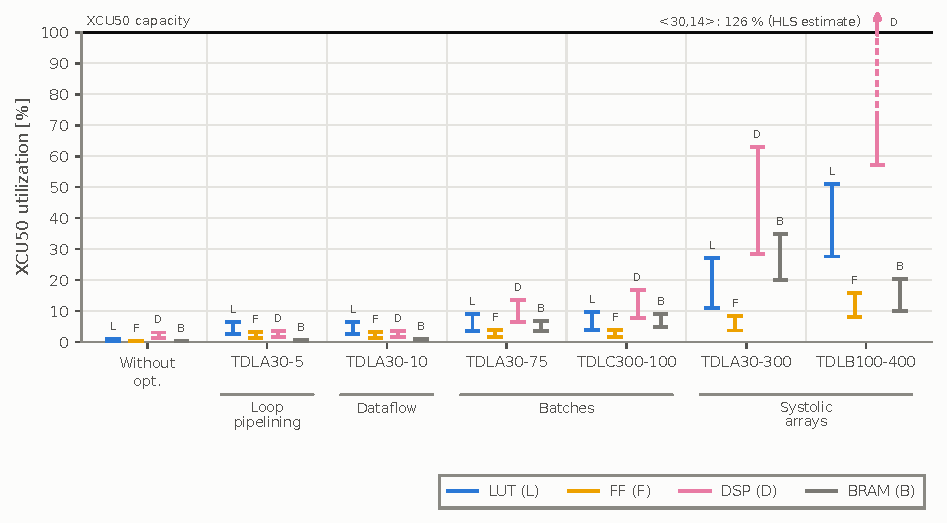
\includegraphics[width=\textwidth]{Images/RESULTADOS/recursos_faixa_arquitetura.pdf}
\vspace{4pt}
\legend{\textcolor{red}{Fonte: a autora. Circuito $16 \times 16$. No DSP da TDLB100-400, a seta indica que o $\langle 30,14\rangle$ passa da capacidade do XCU50: a estimativa do HLS é de 126\%, e ele não cabe no FPGA.}}
\end{figure}

% ---------------------------------------------------------------------
\subsubsection{\texorpdfstring{\textcolor{red}{Pipeline de laços}}{Pipeline de laços}}\label{subsubsec:resultados-pipeline-lacos}
% ---------------------------------------------------------------------
\textcolor{red}{Na versão sem otimização, o recurso mais usado são os DSPs, com 1,4 a 3,1\%. A arquitetura da TDLA30-5 reduz o intervalo de 3,6 a 4,5 vezes. Os DSPs crescem só de 1,1 a 1,2 vez, mas as LUTs crescem de 4,6 a 6,8 vezes, e os FFs, de 9,4 a 13,2 vezes. Com isso, o recurso mais usado passa a ser a LUT, com 2,5 a 6,6\%.}

\textcolor{red}{Esse aumento vem dos divisores. No relatório do HLS, os divisores da versão sem otimização são sequenciais: cada um faz uma divisão por vez e só aceita a próxima quando termina. Com o pipeline de laços, o laço da divisão começa uma iteração por ciclo, e o HLS usa divisores em pipeline, que aceitam uma divisão por ciclo. O único relatório do HLS com o uso de cada operador dessa arquitetura é o de palavras de 24 bits. Nele, os quatro divisores da LU e da substituição direta somam 91\% dos FFs e 71\% das LUTs, e nenhum DSP.}

% ---------------------------------------------------------------------
\subsubsection{\texorpdfstring{\textcolor{red}{Dataflow entre etapas}}{Dataflow entre etapas}}\label{subsubsec:resultados-dataflow}
% ---------------------------------------------------------------------
\textcolor{red}{A arquitetura da TDLA30-10 reduz o intervalo mais 2,5 a 2,7 vezes, e as LUTs, os FFs e os DSPs não mudam. O dataflow não cria operadores novos (Seção~\ref{subsubsec:hw-dataflow}). O custo fica na memória, e as BRAMs crescem de 1,3 a 1,7 vez. Entre as etapas, o HLS usa buffers ping-pong, que guardam cada matriz pelo menos duas vezes~\cite[p.~115]{kastner-hls}. Como os divisores são os mesmos, o recurso mais usado continua sendo a LUT, com 2,5 a 6,5\%.}

% ---------------------------------------------------------------------
\subsubsection{\texorpdfstring{\textcolor{red}{Lotes de matrizes}}{Lotes de matrizes}}\label{subsubsec:resultados-lotes}
% ---------------------------------------------------------------------
\textcolor{red}{Com lote, as BRAMs seguem o número de bancos de memória, e não o número de matrizes guardadas. Cada banco ocupa pelo menos um bloco de BRAM, mesmo quando guarda poucas palavras.}

\textcolor{red}{Na TDLA30-75, com 6 cópias, o intervalo por matriz é de 5,7 a 6,3 vezes menor que na TDLA30-10. Os DSPs crescem de 3,6 a 3,8 vezes, e as LUTs, só de 1,3 a 1,5 vez. Os multiplicadores das atualizações são copiados 6 vezes, mas o divisor de cada etapa é um só para as cópias (Seção~\ref{subsubsec:hw-lotes}). Assim, a parte do circuito que mais usa LUTs não é copiada. As BRAMs crescem de 6,9 a 8,2 vezes, porque cada matriz passa a ficar em 6 bancos, um por cópia. Da TDLA30-75 para a TDLC300-100, as cópias vão de 6 para 8, e as BRAMs crescem na mesma proporção, 1,33 vez, em todos os formatos.}

\textcolor{red}{Assim, a BRAM e os DSPs ficam próximos, e o recurso mais usado depende do formato. Do $\langle 20,8\rangle$ ao $\langle 24,12\rangle$, é a BRAM, com 6,7\% na TDLA30-75 e 8,9\% na TDLC300-100. No $\langle 18,8\rangle$, essas arquiteturas usam cerca de metade das BRAMs dos outros formatos, e a partir do $\langle 26,12\rangle$, os DSPs crescem. Nesses formatos, o recurso mais usado são os DSPs.}

% DSP x formato (2026-11-13): larguras dos multiplicadores nos RTL dos pacotes (pacote_servidor_formatos*/
%   versoes/<fmt>_<arq>/rtl/*mul_*): 28 (<18,8>), 32 (<20,8>, <22,12>), 36 (<24,12>), 40 (<26,12>),
%   42 (<28,14>), 46 (<30,14>) bits; iguais na 606 e na 152. DSPs por multiplicador no csynth.rpt:
%   mul_36s_36s = 4 (cholesky_hardware_diretivas_606/sintese, pacote_servidor_2023/_montagem/152);
%   mul_46s_46s = 9 (viabilidade_30_14/152_sistolico). Sem relatório com DSPs por multiplicador em 40 e 42 bits.
%   UG1399 p. 499 (página do PDF): multiplicação mais larga que o necessário usa vários módulos DSP.
\textcolor{red}{Os DSPs crescem com o formato porque os multiplicadores ficam mais largos. Nos relatórios do HLS, os operandos dos multiplicadores das atualizações têm 28 bits no $\langle 18,8\rangle$, 36 bits no $\langle 24,12\rangle$ e 46 bits no $\langle 30,14\rangle$. Uma multiplicação mais larga é feita com vários DSPs~\cite[p.~499]{ug1399}. Do $\langle 18,8\rangle$ ao $\langle 24,12\rangle$, o total de DSPs quase não muda, e no relatório do $\langle 24,12\rangle$ cada multiplicador usa 4 DSPs. A partir do $\langle 26,12\rangle$, com 40 bits, o total cresce. No $\langle 30,14\rangle$, cada multiplicador usa 9 DSPs.}

% ---------------------------------------------------------------------
\subsubsection{\texorpdfstring{\textcolor{red}{Arranjos sistólicos}}{Arranjos sistólicos}}\label{subsubsec:resultados-sistolico}
% ---------------------------------------------------------------------
\textcolor{red}{Na TDLA30-300, com só 2 cópias, o intervalo é de 3,0 a 3,3 vezes menor que na TDLC300-100. Em cada etapa, as 2 cópias somam 32 multiplicadores, um por PE, contra 8 na TDLC300-100, e cada cópia tem o seu divisor (Seção~\ref{subsubsec:hw-sistolico}). Os DSPs crescem de 3,7 a 3,8 vezes, e as LUTs, de 2,7 a 2,9 vezes. Cada linha da matriz fica em 16 bancos, um por PE, e cada cópia tem os seus. Assim, as BRAMs crescem de 3,8 a 4,2 vezes. No relatório do HLS de palavras de 24 bits, cada um desses bancos ocupa um bloco de 18~Kb, mas guarda só 256 palavras, cerca de um terço do bloco. Como na TDLC300-100, o recurso mais usado é a BRAM do $\langle 20,8\rangle$ ao $\langle 24,12\rangle$, com 34,2 a 34,4\%, e os DSPs nos outros formatos. Os multiplicadores são os mesmos dos lotes, e os DSPs crescem com o formato pelo mesmo motivo (Seção~\ref{subsubsec:resultados-lotes}). Mas, como a TDLA30-300 já usa muitos DSPs, esse crescimento pesa mais no FPGA: os DSPs vão de 28,6\% no $\langle 24,12\rangle$ para 63,1\% no $\langle 30,14\rangle$.}

\textcolor{red}{Na TDLB100-400, as cópias vão de 2 para 4, e o intervalo cai à metade, de 128 para 64 ciclos. Os DSPs também dobram. As LUTs crescem de 2,4 a 2,5 vezes, e as BRAMs caem quase à metade. Com 4 cópias, cada banco guarda metade das palavras, e o HLS fez esses bancos em LUTs, e não em BRAM. Uma memória pode ser feita em BRAM, em LUTs (LUTRAM) ou em URAM~\cite[p.~53]{ug1399}. No relatório do Vivado, as LUTs usadas como memória crescem de 7,4 a 9,8 vezes, e as LUTs de lógica, 2,0 vezes, como as cópias. Assim, em todos os formatos, o recurso mais usado são os DSPs, com 57,1 a 72,4\%, e as BRAMs ficam entre 10,0 e 20,2\%.}

% ---------------------------------------------------------------------
\subsection{\texorpdfstring{\textcolor{red}{Comparação entre as arquiteturas}}{Comparação entre as arquiteturas}}\label{subsec:resultados-recursos}
% ---------------------------------------------------------------------
% FONTE: resultados_vivado_servidor.csv (relatório de implementação, utilizacao.rpt); totais do
%   XCU50 do próprio utilizacao.rpt: 871.680 LUT, 1.743.360 FF, 5.952 DSP, 1.344 blocos de
%   36 Kb (2.688 de 18 Kb). 7.512 DSP do <30,14> na 114: coluna observacao do CSV.

\textcolor{red}{A Tabela~\ref{tab:recursos-faixa} mostra o melhor e o pior caso de cada arquitetura entre os formatos: o menor e o maior uso de cada recurso, de caminho crítico e de intervalo entre inversões. Os valores de cada formato estão nas Tabelas~\ref{tab:recursos} e \ref{tab:recursos-sem-otimizacao} (Apêndice~\ref{ap:recursos}).}

\textcolor{red}{As arquiteturas sem lote (TDLA30-5 e TDLA30-10) usam no máximo 6,6\% de cada recurso, e a versão sem otimização, no máximo 3,1\%. Em $32 \times 32$, a versão sem otimização usa quase os mesmos recursos que em $16 \times 16$, mas o intervalo cresce de 5 a 6 vezes.}

\begin{table}[htbp]
\caption{\textcolor{red}{Menor e maior uso de recursos, caminho crítico e intervalo entre inversões de cada arquitetura, entre os formatos.}}
\label{tab:recursos-faixa}
\vspace{4pt} % a classe zera o espaço entre a caption e a tabela
\centering
\footnotesize
\color{red}
\renewcommand{\arraystretch}{1.2}
\setlength{\tabcolsep}{2pt}
\begin{tabular}{lccccccc}
\toprule
\textbf{Test condition} & \textbf{LUT (\%)} & \textbf{FF (\%)} & \textbf{DSP (\%)} & \textbf{BRAM (\%)} & \begin{tabular}[c]{@{}c@{}}\textbf{Critical}\\\textbf{path (ns)}\end{tabular} & \begin{tabular}[c]{@{}c@{}}\textbf{Interval}\\\textbf{(cycles)}\end{tabular} & \begin{tabular}[c]{@{}c@{}}\textbf{Limit}\\\textbf{(cycles)}\end{tabular} \\
\midrule
TDLA30-5 & 2.5--6.6 & 1.2--3.2 & 1.7--3.7 & 0.4--0.6 & 7.24--9.03 & 7,081--8,627 & 9,090 \\
TDLA30-10 & 2.5--6.5 & 1.2--3.3 & 1.7--3.7 & 0.5--0.9 & 7.54--8.36 & 2,765--3,320 & 4,545 \\
TDLA30-75 & 3.7--9.0 & 1.6--4.0 & 6.3--13.5 & 3.6--6.7 & 7.87--8.98 & 483.9--528.9 & 606 \\
TDLC300-100 & 4.0--9.7 & 1.6--4.0 & 7.7--16.9 & 4.8--8.9 & 7.79--9.37 & 387.3--421.1 & 454 \\
TDLA30-300 & 11.0--27.2 & 3.7--8.5 & 28.6--63.1 & 20.0--35.0 & 8.73--9.66 & 128 & 151 \\
TDLB100-400 & 27.6--51.0 & 8.0--15.9 & 57.1--72.4 & 10.0--20.2 & 9.38--9.74 & 64 & 113 \\
\midrule
Without opt., 16 $\times$ 16 & 0.5--1.0 & 0.1--0.2 & 1.4--3.1 & 0.3--0.5 & 7.80--9.15 & 26,702--38,567 & -- \\
Without opt., 32 $\times$ 32 & 0.5--1.0 & 0.1--0.3 & 1.4--3.1 & 0.3--0.7 & 7.72--8.58 & 159,086--194,367 & -- \\
\bottomrule
\end{tabular}
\vspace{4pt}
\legend{\textcolor{red}{Fonte: a autora. Recursos em porcentagem do XCU50. Em quase todos os casos, o menor valor vem do $\langle 18,8\rangle$ e o maior, do $\langle 30,14\rangle$ ($\langle 28,14\rangle$ na TDLB100-400). O caminho crítico não segue essa ordem. Em $32 \times 32$, sem o intervalo do $\langle 18,8\rangle$ e do $\langle 20,8\rangle$, que não foram medidos.}}
\end{table}

\textcolor{red}{A Tabela~\ref{tab:recurso-mais-usado} mostra o recurso mais usado em cada formato. O maior efeito do formato está no $\langle 30,14\rangle$, em que os DSPs quase dobram em relação ao $\langle 28,14\rangle$: na TDLA30-300, vão de 36 para 63\%. Na TDLB100-400, o $\langle 30,14\rangle$ não cabe no FPGA: a estimativa do HLS é de 7.512 DSPs, e o XCU50 tem 5.952.}

\begin{table}[htbp]
\caption{\textcolor{red}{Recurso mais usado do XCU50, em porcentagem, por formato e arquitetura.}}
\label{tab:recurso-mais-usado}
\vspace{4pt} % a classe zera o espaço entre a caption e a tabela
\centering
\footnotesize
\color{red}
\renewcommand{\arraystretch}{1.2}
\setlength{\tabcolsep}{4pt}
\begin{tabular}{lcccccccc}
\toprule
\textbf{Test condition} & \textbf{$\langle 18,8\rangle$} & \textbf{$\langle 18,8\rangle$$^{*}$} & \textbf{$\langle 20,8\rangle$} & \textbf{$\langle 22,12\rangle$} & \textbf{$\langle 24,12\rangle$} & \textbf{$\langle 26,12\rangle$} & \textbf{$\langle 28,14\rangle$} & \textbf{$\langle 30,14\rangle$$^{*}$} \\
\midrule
TDLA30-5 & 2.5 (L) & 2.6 (L) & 3.2 (L) & 3.2 (L) & 4.1 (L) & 4.9 (L) & 5.4 (L) & 6.6 (L) \\
TDLA30-10 & 2.5 (L) & 2.6 (L) & 3.2 (L) & 3.3 (L) & 4.1 (L) & 5.0 (L) & 5.5 (L) & 6.5 (L) \\
TDLA30-75 & 6.3 (D) & 6.3 (D) & 6.7 (B) & 6.7 (B) & 6.7 (B) & 7.7 (D) & 7.9 (D) & 13.5 (D) \\
TDLC300-100 & 7.7 (D) & 7.7 (D) & 8.9 (B) & 8.9 (B) & 8.9 (B) & 9.4 (D) & 9.7 (D) & 16.9 (D) \\
TDLA30-300 & 28.6 (D) & 28.6 (D) & 34.2 (B) & 34.3 (B) & 34.4 (B) & 35.1 (D) & 36.2 (D) & 63.1 (D) \\
TDLB100-400 & 57.2 (D) & 57.2 (D) & 57.6 (D) & 57.3 (D) & 57.1 (D) & 70.3 (D) & 72.4 (D) & -- \\
\bottomrule
\end{tabular}
\vspace{4pt}
\legend{\textcolor{red}{Fonte: a autora. Entre parênteses, o recurso: L = LUT, D = DSP, B = BRAM. $^{*}$\texttt{AP\_TRN}/\texttt{AP\_SAT}; os outros, \texttt{AP\_RND\_ZERO}/\texttt{AP\_WRAP}. --: não cabe no FPGA.}}
\end{table}

% Ocupação formato a formato (tab:recurso-mais-usado): TDLA30-10 -> TDLA30-75 cresce 1,4 a 2,5 vezes;
%   TDLA30-300 -> TDLB100-400, 1,7 a 2,0 vezes.
\textcolor{red}{O gráfico da esquerda da Figura~\ref{fig:potencia-recursos} mostra o recurso mais usado. Como ele muda de uma arquitetura para outra, a ocupação não segue o limite de ciclos. Da TDLA30-10 para a TDLA30-75, o limite fica 7,5 vezes menor, e a ocupação cresce só de 1,4 a 2,5 vezes. Da TDLA30-300 para a TDLB100-400, o limite fica só 1,3 vez menor, e a ocupação cresce de 1,7 a 2,0 vezes.}

% ---------------------------------------------------------------------
\subsection{\texorpdfstring{\textcolor{red}{Potência e energia}}{Potência e energia}}\label{subsec:resultados-potencia}
% ---------------------------------------------------------------------
% FONTE: resultados_vivado_servidor.csv (report_power com SAIF); estática = total - dinâmica
%   (2,212 a 2,300 W em todas as linhas 16 x 16). Inclinação e razões: tabelas/resumo.txt.
%   Figura da potência média no ritmo (potencia_media_condicao) retirada em 2026-11-09, a
%   pedido da autora: a de potência dinâmica já mostra esses dados.

% Razão TDLB100-400 / TDLA30-5 formato a formato: 15,4 (<28,14>) a 20,0 (<18,8> TRN/SAT).
\textcolor{red}{A Tabela~\ref{tab:potencia-dinamica} mostra a potência dinâmica. Em cada formato, a da TDLB100-400 é de 15 a 20 vezes a da TDLA30-5. O formato pesa menos que a arquitetura. Do $\langle 18,8\rangle$ ao $\langle 28,14\rangle$, a potência dinâmica cresce de 1,6 a 2,0 vezes em cada arquitetura. Nesse intervalo, cada bit a mais na palavra custa, em média, 15~mW na TDLA30-5 e 180~mW na TDLB100-400. A potência estática fica entre 2,21 e 2,30~W em todas as arquiteturas e formatos.}


\begin{table}[htbp]
\caption{\textcolor{red}{Potência dinâmica, em W, por formato e arquitetura.}}
\label{tab:potencia-dinamica}
\vspace{4pt} % a classe zera o espaço entre a caption e a tabela
\centering
\footnotesize
\color{red}
\renewcommand{\arraystretch}{1.2}
\setlength{\tabcolsep}{3pt}
\begin{tabular}{lcccccccc}
\toprule
\textbf{Test condition} & \textbf{$\langle 18,8\rangle$} & \textbf{$\langle 18,8\rangle$$^{*}$} & \textbf{$\langle 20,8\rangle$} & \textbf{$\langle 22,12\rangle$} & \textbf{$\langle 24,12\rangle$} & \textbf{$\langle 26,12\rangle$} & \textbf{$\langle 28,14\rangle$} & \textbf{$\langle 30,14\rangle$$^{*}$} \\
\midrule
TDLA30-5 & 0.151 & 0.158 & 0.187 & 0.194 & 0.234 & 0.280 & 0.305 & 0.377 \\
TDLA30-10 & 0.209 & 0.208 & 0.252 & 0.253 & 0.305 & 0.362 & 0.391 & 0.496 \\
TDLA30-75 & 0.369 & 0.400 & 0.450 & 0.474 & 0.546 & 0.618 & 0.647 & 0.868 \\
TDLC300-100 & 0.452 & 0.482 & 0.570 & 0.573 & 0.666 & 0.759 & 0.805 & 1.037 \\
TDLA30-300 & 1.368 & 1.425 & 1.679 & 1.753 & 1.973 & 2.087 & 2.180 & 3.065 \\
TDLB100-400 & 2.908 & 3.167 & 3.313 & 3.477 & 4.062 & 4.456 & 4.703 & -- \\
\midrule
Without opt., 16 $\times$ 16 & 0.031 & 0.034 & 0.035 & 0.037 & 0.041 & 0.046 & 0.048 & 0.059 \\
Without opt., 32 $\times$ 32 & -- & -- & -- & 0.040 & 0.046 & 0.051 & 0.053 & 0.065 \\
\bottomrule
\end{tabular}
\vspace{4pt}
\legend{\textcolor{red}{Fonte: a autora. Arquitetura de cada condição de teste em $16 \times 16$. $^{*}$\texttt{AP\_TRN}/\texttt{AP\_SAT}; os outros, \texttt{AP\_RND\_ZERO}/\texttt{AP\_WRAP}. --: sem medida ou não cabe no FPGA.}}
\end{table}

% Faixas formato a formato (resultados_vivado_servidor.csv): com lote 1,75 a 4,59 uJ; TDLA30-5 /
%   maior e menor com lote no mesmo formato: 5,7 a 8,8; TDLA30-10 / TDLA30-5: 0,50 a 0,54.
\textcolor{red}{A Tabela~\ref{tab:energia-inversao} e a Figura~\ref{fig:energia-inversao} mostram a energia por inversão. Nas arquiteturas com lote, ela fica entre 1,75 e 4,59~$\mu$J, e as quatro ficam próximas em cada formato. A da TDLA30-5 gasta de 5,7 a 8,8 vezes mais que elas, no mesmo formato. Ela tem a menor potência dinâmica, mas cada inversão leva de 7.081 a 8.627 ciclos, contra 64 a 529 nas arquiteturas com lote. A da TDLA30-10 gasta cerca de metade da TDLA30-5.}


\begin{table}[htbp]
\caption{\textcolor{red}{Energia por inversão, em $\mu$J, por formato e arquitetura.}}
\label{tab:energia-inversao}
\vspace{4pt} % a classe zera o espaço entre a caption e a tabela
\centering
\footnotesize
\color{red}
\renewcommand{\arraystretch}{1.2}
\setlength{\tabcolsep}{3pt}
\begin{tabular}{lcccccccc}
\toprule
\textbf{Test condition} & \textbf{$\langle 18,8\rangle$} & \textbf{$\langle 18,8\rangle$$^{*}$} & \textbf{$\langle 20,8\rangle$} & \textbf{$\langle 22,12\rangle$} & \textbf{$\langle 24,12\rangle$} & \textbf{$\langle 26,12\rangle$} & \textbf{$\langle 28,14\rangle$} & \textbf{$\langle 30,14\rangle$$^{*}$} \\
\midrule
TDLA30-5 & 10.69 & 11.60 & 13.74 & 14.25 & 17.77 & 21.96 & 24.66 & 32.52 \\
TDLA30-10 & 5.81 & 5.75 & 7.31 & 7.34 & 9.21 & 11.37 & 12.51 & 16.47 \\
TDLA30-75 & 1.79 & 1.94 & 2.22 & 2.34 & 2.75 & 3.18 & 3.36 & 4.59 \\
TDLC300-100 & 1.75 & 1.87 & 2.25 & 2.26 & 2.68 & 3.11 & 3.33 & 4.37 \\
TDLA30-300 & 1.75 & 1.82 & 2.15 & 2.24 & 2.52 & 2.67 & 2.79 & 3.92 \\
TDLB100-400 & 1.86 & 2.03 & 2.12 & 2.23 & 2.60 & 2.85 & 3.01 & -- \\
\midrule
Without opt., 16 $\times$ 16 & 8.28 & 9.09 & 10.64 & 11.25 & 13.31 & 15.81 & 17.00 & 22.75 \\
Without opt., 32 $\times$ 32 & -- & -- & -- & 63.63 & 76.96 & 89.24 & 94.92 & 126.34 \\
\bottomrule
\end{tabular}
\vspace{4pt}
\legend{\textcolor{red}{Fonte: a autora. Cálculo na Seção~\ref{subsec:hw-potencia}. $^{*}$\texttt{AP\_TRN}/\texttt{AP\_SAT}; os outros, \texttt{AP\_RND\_ZERO}/\texttt{AP\_WRAP}. --: sem medida ou não cabe no FPGA.}}
\end{table}

\begin{figure}[!ht]
\caption{\textcolor{red}{Energia por inversão por formato e condição de teste.}}
\label{fig:energia-inversao}
\vspace{4pt} % a classe zera o espaço entre a caption e a figura
\centering
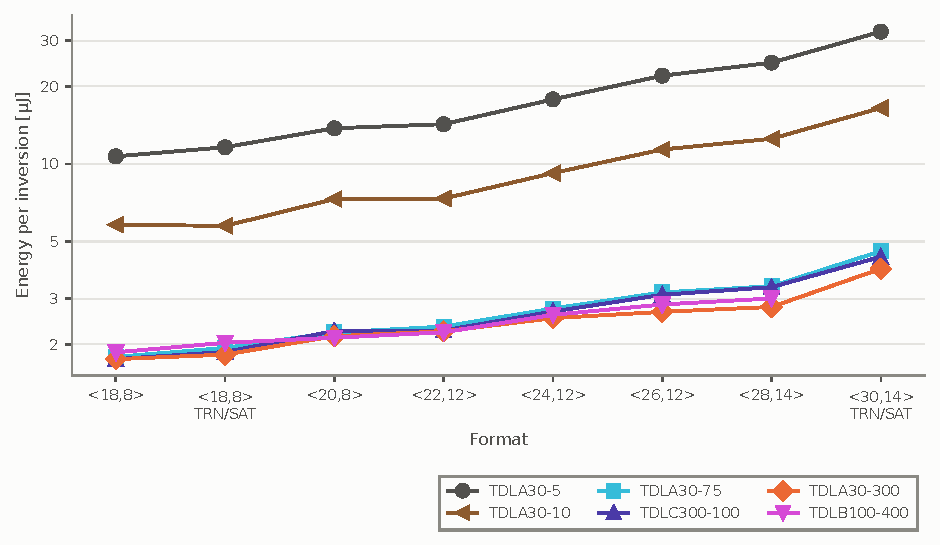
\includegraphics[width=\textwidth]{Images/RESULTADOS/energia_inversao.pdf}
\vspace{4pt}
\legend{\textcolor{red}{Fonte: a autora. Eixo vertical em escala logarítmica. Sem TRN/SAT no rótulo, o formato usa \texttt{AP\_RND\_ZERO}/\texttt{AP\_WRAP}. O $\langle 30,14\rangle$ da TDLB100-400 não cabe no FPGA.}}
\end{figure}

% FONTE: potencia_recursos_lado_data.csv (dinamica_sobre_estatica_pct, ocupacao_pct).
\textcolor{red}{A Figura~\ref{fig:potencia-recursos} junta, por formato, a ocupação do recurso mais usado (Tabela~\ref{tab:recurso-mais-usado}) e a potência dinâmica. Da TDLA30-5 à TDLC300-100, a potência dinâmica fica entre 7 e 46\% da estática. Na TDLA30-300, ela vai de 61 a 135\%, e na TDLB100-400, de 128 a 204\%.}


\begin{figure}[!ht]
\caption{\textcolor{red}{Ocupação do recurso mais usado do XCU50 (esquerda) e potência dinâmica (direita), por formato e condição de teste.}}
\label{fig:potencia-recursos}
\vspace{4pt} % a classe zera o espaço entre a caption e a figura
\centering
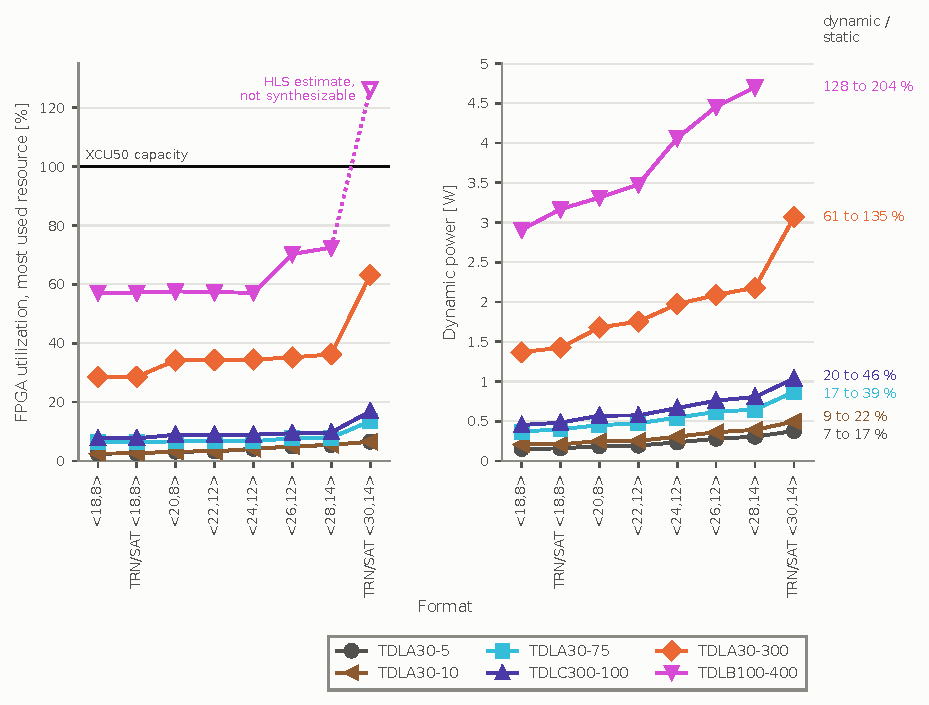
\includegraphics[width=\textwidth]{Images/RESULTADOS/potencia_recursos.pdf}
\vspace{4pt}
\legend{\textcolor{red}{Fonte: a autora. À direita, a potência dinâmica em porcentagem da estática, do menor ao maior formato. No $\langle 30,14\rangle$ da TDLB100-400, a ocupação é a estimativa do HLS.}}
\end{figure}
